\documentclass[tikz]{standalone}
\usepackage{xcolor}
\definecolor{bg}{HTML}{171D2B}
\definecolor{aksen}{HTML}{F7B538}
\definecolor{garis}{HTML}{E2E8F0}
\pagecolor{bg}
\begin{document}
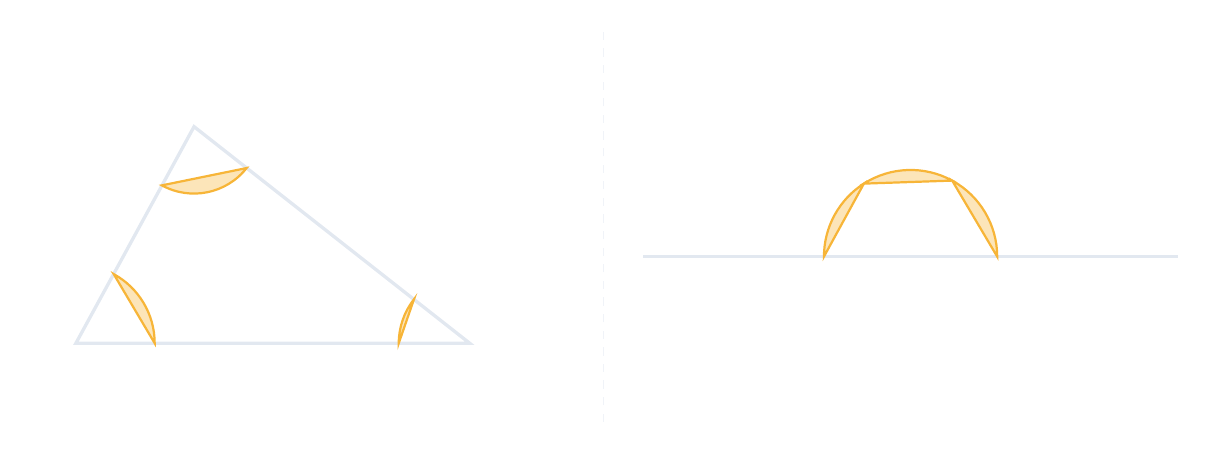
\begin{tikzpicture}[
  scale=1,
  every node/.style={text=white, font=\Large},
  arcseg/.style={draw=aksen, fill=aksen!35, thick}
]
% --- Kiri: segitiga ABC dengan sudut ---
\coordinate (A) at (0,0);
\coordinate (B) at (5,0);
\coordinate (C) at (1.5,2.75);
\draw[very thick, garis] (A) -- (B) -- (C) -- cycle;
% sudut di A: arctan(2.75/1.5) = 61.3
\draw[arcseg] (A) ++(0:1.0) arc (0:61.3:1.0) -- cycle;
\node at (28:1.5) {$\alpha$};
% sudut di B: dari 180 menuju arah C (141.8)
\draw[arcseg] (B) ++(180:0.9) arc (180:141.8:0.9) -- cycle;
\node at ([shift={(B)}]162:1.4) {$\gamma$};
% sudut di C: antara arah ke A (241.3) dan ke B (321.8)
\draw[arcseg] (C) ++(241.3:0.85) arc (241.3:321.8:0.85) -- cycle;
\node at ([shift={(C)}]281:1.4) {$\beta$};
\node[below left] at (A) {$A$};
\node[below right] at (B) {$B$};
\node[above] at (C) {$C$};

% garis pemisah
\draw[garis!50, dashed] (6.7,-1) -- (6.7,4);

% --- Kanan: tiga sudut disusun di garis lurus pada O (61.3 + 61.3 + 57.4 = 180) ---
\begin{scope}[shift={(10.6,1.1)}]
  \draw[very thick, garis] (-3.4,0) -- (3.4,0);
  \coordinate (O) at (0,0);
  \draw[arcseg] (O) ++(0:1.1) arc (0:61.3:1.1) -- cycle;
  \draw[arcseg] (O) ++(61.3:1.1) arc (61.3:122.6:1.1) -- cycle;
  \draw[arcseg] (O) ++(122.6:1.1) arc (122.6:180:1.1) -- cycle;
  \node at (30:1.6) {$\alpha$};
  \node at (91:1.6) {$\beta$};
  \node at (152:1.6) {$\gamma$};
  \node[below=2mm] at (O) {$O$};
\end{scope}
\end{tikzpicture}
\end{document}
